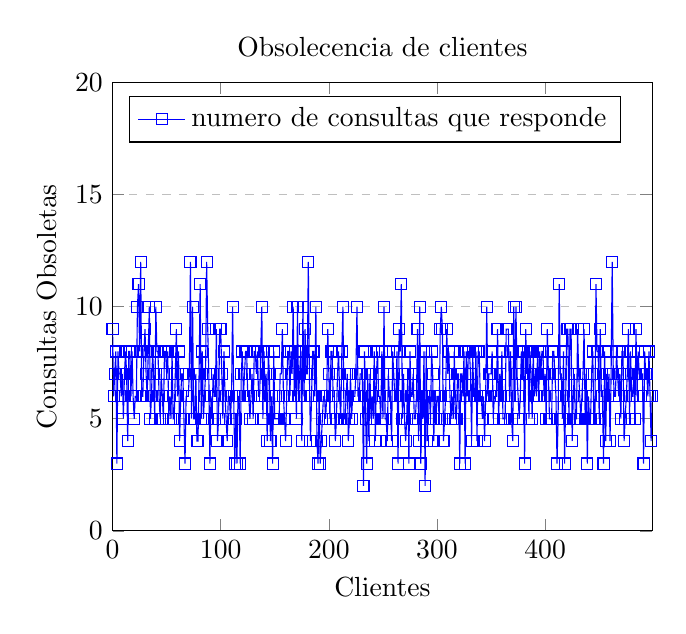
\begin{tikzpicture}
\begin{axis}[
    title={Obsolecencia de clientes},
    xlabel={Clientes},
    ylabel={Consultas Obsoletas},
    xmin=0, xmax=499,
    ymin=0, ymax=20,
    xtick={},
    ytick={},
    legend pos=north west,
    ymajorgrids=true,
    grid style=dashed,
]

\addplot[
    color=blue,
    mark=square,
    ]
    coordinates {
%OBSOLECENCIA CLIENTE RESPECTO A LA REGION DE ENCUBRIMIENTO
(0,9)
(1,6)
(2,7)
(3,8)
(4,3)
(5,8)
(6,7)
(7,7)
(8,6)
(9,7)
(10,5)
(11,7)
(12,8)
(13,7)
(14,4)
(15,8)
(16,8)
(17,6)
(18,8)
(19,6)
(20,5)
(21,6)
(22,6)
(23,10)
(24,11)
(25,8)
(26,12)
(27,6)
(28,6)
(29,8)
(30,9)
(31,7)
(32,6)
(33,8)
(34,10)
(35,5)
(36,6)
(37,8)
(38,7)
(39,5)
(40,10)
(41,8)
(42,8)
(43,6)
(44,5)
(45,7)
(46,6)
(47,5)
(48,8)
(49,8)
(50,7)
(51,8)
(52,5)
(53,6)
(54,5)
(55,8)
(56,5)
(57,5)
(58,7)
(59,9)
(60,6)
(61,8)
(62,4)
(63,6)
(64,7)
(65,7)
(66,5)
(67,3)
(68,6)
(69,6)
(70,6)
(71,7)
(72,12)
(73,5)
(74,10)
(75,5)
(76,5)
(77,7)
(78,4)
(79,4)
(80,7)
(81,11)
(82,5)
(83,8)
(84,5)
(85,6)
(86,7)
(87,12)
(88,9)
(89,7)
(90,3)
(91,6)
(92,5)
(93,7)
(94,6)
(95,6)
(96,9)
(97,4)
(98,5)
(99,9)
(100,9)
(101,7)
(102,5)
(103,8)
(104,6)
(105,5)
(106,4)
(107,6)
(108,6)
(109,5)
(110,6)
(111,10)
(112,6)
(113,3)
(114,5)
(115,3)
(116,6)
(117,6)
(118,3)
(119,7)
(120,8)
(121,6)
(122,7)
(123,8)
(124,8)
(125,6)
(126,6)
(127,5)
(128,6)
(129,7)
(130,5)
(131,8)
(132,8)
(133,7)
(134,8)
(135,6)
(136,6)
(137,8)
(138,10)
(139,5)
(140,8)
(141,6)
(142,7)
(143,4)
(144,8)
(145,7)
(146,4)
(147,6)
(148,3)
(149,8)
(150,5)
(151,5)
(152,5)
(153,5)
(154,5)
(155,7)
(156,7)
(157,9)
(158,6)
(159,5)
(160,4)
(161,6)
(162,8)
(163,8)
(164,6)
(165,8)
(166,7)
(167,10)
(168,6)
(169,8)
(170,5)
(171,10)
(172,6)
(173,7)
(174,8)
(175,4)
(176,10)
(177,6)
(178,9)
(179,7)
(180,7)
(181,12)
(182,7)
(183,4)
(184,6)
(185,8)
(186,8)
(187,6)
(188,10)
(189,4)
(190,3)
(191,6)
(192,3)
(193,4)
(194,5)
(195,6)
(196,6)
(197,5)
(198,6)
(199,9)
(200,7)
(201,5)
(202,8)
(203,8)
(204,6)
(205,6)
(206,4)
(207,5)
(208,7)
(209,8)
(210,6)
(211,5)
(212,8)
(213,10)
(214,5)
(215,5)
(216,6)
(217,7)
(218,4)
(219,5)
(220,7)
(221,5)
(222,6)
(223,6)
(224,6)
(225,7)
(226,10)
(227,6)
(228,6)
(229,7)
(230,7)
(231,7)
(232,2)
(233,8)
(234,5)
(235,3)
(236,7)
(237,4)
(238,7)
(239,5)
(240,6)
(241,5)
(242,8)
(243,4)
(244,7)
(245,8)
(246,6)
(247,6)
(248,5)
(249,8)
(250,5)
(251,10)
(252,5)
(253,5)
(254,4)
(255,7)
(256,6)
(257,6)
(258,4)
(259,8)
(260,7)
(261,6)
(262,6)
(263,8)
(264,3)
(265,9)
(266,8)
(267,11)
(268,5)
(269,7)
(270,5)
(271,4)
(272,5)
(273,7)
(274,3)
(275,8)
(276,6)
(277,6)
(278,7)
(279,5)
(280,5)
(281,6)
(282,9)
(283,4)
(284,10)
(285,3)
(286,6)
(287,5)
(288,8)
(289,2)
(290,8)
(291,4)
(292,6)
(293,6)
(294,5)
(295,8)
(296,7)
(297,4)
(298,6)
(299,5)
(300,6)
(301,6)
(302,5)
(303,9)
(304,10)
(305,9)
(306,4)
(307,5)
(308,6)
(309,9)
(310,7)
(311,8)
(312,6)
(313,5)
(314,6)
(315,5)
(316,8)
(317,5)
(318,5)
(319,7)
(320,7)
(321,3)
(322,7)
(323,7)
(324,6)
(325,8)
(326,3)
(327,8)
(328,6)
(329,8)
(330,8)
(331,7)
(332,4)
(333,8)
(334,6)
(335,6)
(336,8)
(337,4)
(338,8)
(339,8)
(340,6)
(341,6)
(342,5)
(343,6)
(344,4)
(345,6)
(346,10)
(347,6)
(348,7)
(349,7)
(350,7)
(351,8)
(352,5)
(353,6)
(354,6)
(355,6)
(356,9)
(357,5)
(358,7)
(359,6)
(360,8)
(361,5)
(362,5)
(363,5)
(364,9)
(365,9)
(366,9)
(367,6)
(368,8)
(369,5)
(370,4)
(371,10)
(372,6)
(373,10)
(374,7)
(375,6)
(376,5)
(377,6)
(378,8)
(379,7)
(380,8)
(381,3)
(382,9)
(383,7)
(384,8)
(385,5)
(386,8)
(387,7)
(388,5)
(389,8)
(390,6)
(391,7)
(392,6)
(393,8)
(394,6)
(395,8)
(396,7)
(397,8)
(398,8)
(399,6)
(400,7)
(401,5)
(402,9)
(403,7)
(404,5)
(405,5)
(406,5)
(407,8)
(408,8)
(409,7)
(410,6)
(411,3)
(412,5)
(413,11)
(414,7)
(415,7)
(416,5)
(417,8)
(418,3)
(419,6)
(420,9)
(421,9)
(422,5)
(423,9)
(424,9)
(425,4)
(426,6)
(427,7)
(428,5)
(429,5)
(430,9)
(431,7)
(432,6)
(433,5)
(434,6)
(435,7)
(436,9)
(437,5)
(438,7)
(439,3)
(440,6)
(441,5)
(442,5)
(443,7)
(444,8)
(445,5)
(446,5)
(447,11)
(448,8)
(449,8)
(450,5)
(451,9)
(452,6)
(453,6)
(454,3)
(455,8)
(456,4)
(457,7)
(458,6)
(459,7)
(460,4)
(461,7)
(462,12)
(463,7)
(464,6)
(465,6)
(466,8)
(467,7)
(468,6)
(469,7)
(470,5)
(471,8)
(472,8)
(473,4)
(474,5)
(475,6)
(476,7)
(477,9)
(478,5)
(479,8)
(480,6)
(481,6)
(482,7)
(483,5)
(484,9)
(485,6)
(486,8)
(487,7)
(488,7)
(489,7)
(490,7)
(491,3)
(492,8)
(493,7)
(494,7)
(495,6)
(496,8)
(497,6)
(498,4)
(499,6)
    };
    \legend{numero de consultas que responde}

\end{axis}
\end{tikzpicture}
